%%%%%%%%%%%%%%%%%%%%%%%%%%%%%%%%%%%%%%%%%
% Beamer Presentation
% LaTeX Template
% Version 1.0 (10/11/12)
%
% This template has been downloaded from:
% http://www.LaTeXTemplates.com
%
% License:
% CC BY-NC-SA 3.0 (http://creativecommons.org/licenses/by-nc-sa/3.0/)
%
%%%%%%%%%%%%%%%%%%%%%%%%%%%%%%%%%%%%%%%%%

%----------------------------------------------------------------------------------------
%	PACKAGES AND THEMES
%----------------------------------------------------------------------------------------

\documentclass[10pt]{beamer}

\mode<presentation> {

% The Beamer class comes with a number of default slide themes
% which change the colors and layouts of slides. Below this is a list
% of all the themes, uncomment each in turn to see what they look like.

\renewcommand{\familydefault}{\rmdefault}

\graphicspath{ {./figures/} }
\usepackage{graphicx} % Allows including images
\usepackage{booktabs} % Allows the use of \toprule, \midrule and \bottomrule in tables
\usepackage{tikz} % Allows the use of \toprule, \midrule and \bottomrule in tables
\usepackage{hyperref}
\usepackage{breqn}
\usepackage[printwatermark]{xwatermark}

\usetheme{default}
% \usetheme{AnnArbor}
% \usetheme{Antibes}
% \usetheme{Bergen}
% \usetheme{Berkeley}
% \usetheme{Berlin}
% \usetheme{Boadilla}
% \usetheme{CambridgeUS}
% \usetheme{Copenhagen}
% \usetheme{Darmstadt}
% \usetheme{Dresden}
% \usetheme{Frankfurt}
% \usetheme{Goettingen}
% \usetheme{Hannover}
% \usetheme{Ilmenau}
% \usetheme{JuanLesPins}
% \usetheme{Luebeck}
% \usetheme{Madrid}
% \usetheme{Malmoe}
% \usetheme{Marburg}
% \usetheme{Montpellier}
% \usetheme{PaloAlto}
% \usetheme{Pittsburgh}
% \usetheme{Rochester}
% \usetheme{Singapore}
% \usetheme{Szeged}
% \usetheme{Warsaw}

% As well as themes, the Beamer class has a number of color themes
% for any slide theme. Uncomment each of these in turn to see how it
% changes the colors of your current slide theme.

% \usecolortheme{albatross}
\usecolortheme{beaver}
% \usecolortheme{beetle}
% \usecolortheme{crane}
% \usecolortheme{dolphin}
% \usecolortheme{dove}
% \usecolortheme{fly}
% \usecolortheme{lily}
% \usecolortheme{orchid}
% \usecolortheme{rose}
% \usecolortheme{seagull}
% \usecolortheme{seahorse}
% \usecolortheme{whale}
% \usecolortheme{wolverine}

%\setbeamertemplate{footline} % To remove the footer line in all slides uncomment this line
\setbeamertemplate{footline}[page number] % To replace the footer line in all slides with a simple slide count uncomment this line

\setbeamertemplate{navigation symbols}{} % To remove the navigation symbols from the bottom of all slides uncomment this line

% \setbeamertemplate{background}{
%     \tikz[overlay,remember picture]\node[opacity=0.4]at (current page.center){
%         \includegraphics[width=2cm]{iot_analytics_logo.jpg}
%         }}

}

%----------------------------------------------------------------------------------------
%	TITLE PAGE
%----------------------------------------------------------------------------------------

\title[Is It Getting Sad?]{Exploring the Sentiment of Lyrics from Billboard Top 100 1960-2015} % The short title appears at the bottom of every slide, the full title is only on the title page

\author{Tuomo Kareoja} % Your name
\date{\today} % Date, can be changed to a custom date

\begin{document}

\begin{frame}
\titlepage % Print the title page as the first slide
\end{frame}

\begin{frame}
\frametitle{Agenda} % Table of contents slide, comment this block out to remove it
\tableofcontents % Throughout your presentation, if you choose to use \section{} and \subsection{} commands, these will automatically be printed on this slide as an overview of your presentation
\end{frame}

%----------------------------------------------------------------------------------------
%	PRESENTATION SLIDES
%----------------------------------------------------------------------------------------

%------------------------------------------------
\section{Getting the Data}
%------------------------------------------------

\begin{frame}
\frametitle{
    WebScraping
}

\begin{itemize}
    \item Reading the contents from HTML tables with the BeautifulSoup package
\end{itemize}

{
    \centering
    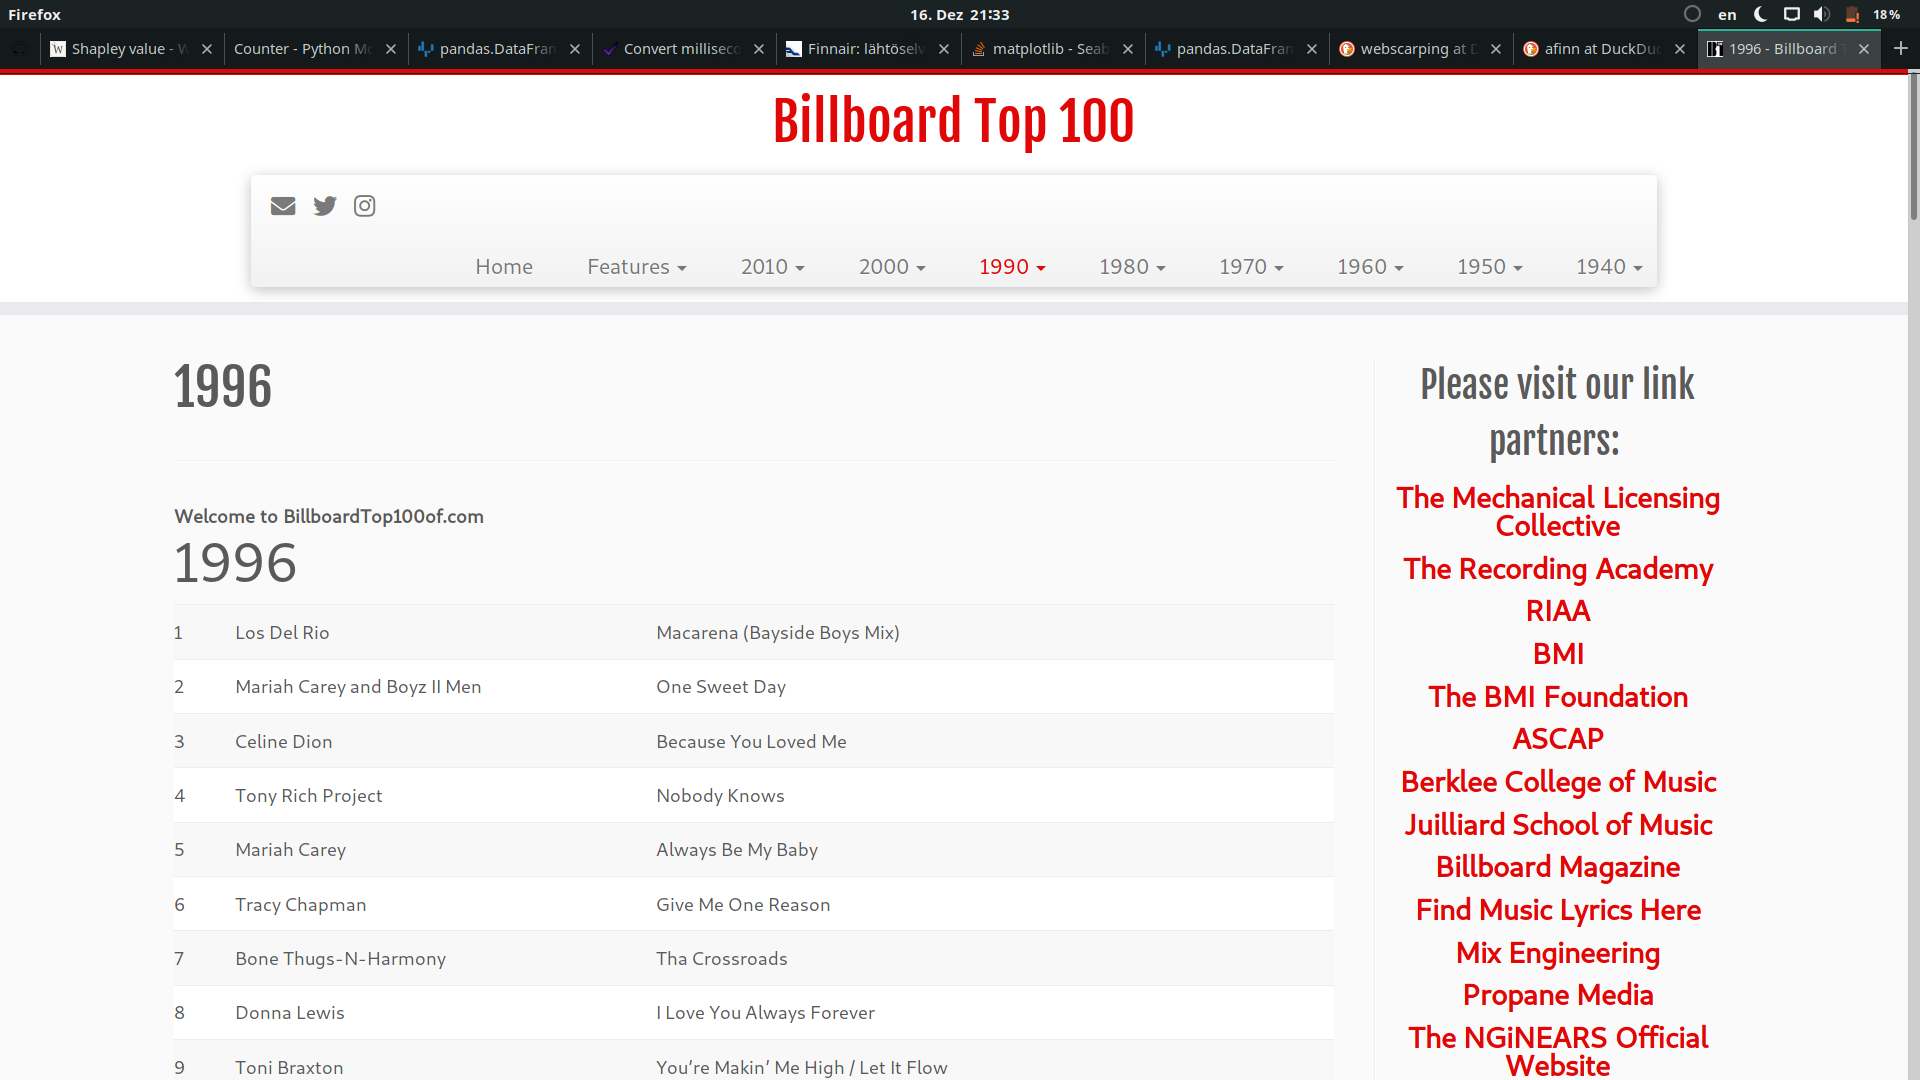
\includegraphics[width=\textwidth, height=\textheight,keepaspectratio]{billboard_top100.png}
    \par
}

\end{frame}

\begin{frame}
\frametitle{Lyrics From APIs}

\begin{itemize}
    \item Used three different APIs with the Requests package
    \begin{enumerate}
        \item Mourits Lyrics (best, but so much down!)
        \item Genius Lyrics
        \item ChartLyrics
    \end{enumerate}
    \item If the lyrics is too long, try a different API (no long bible quotes!)
    \item What you get differs from site to site as the lyrics are added by users
\end{itemize}

\end{frame}

\begin{frame}
\frametitle{Get Track Details From Spotify}

\begin{itemize}
    \item Spotify has a really nice API for getting information about
    the actual audio (e.g. length, danceability, tempo, loudness...)
    \item You need to register an app, and the API, is bit fiddly...
    \item But of course there is a python package does most of the work
    for you! (spotipy)
    \item Still need to first find the song ID and then find the audio features
    with this, so multiple calls needed
\end{itemize}

\end{frame}

%------------------------------------------------
\section{Data Cleaning}
%------------------------------------------------

\begin{frame}
\frametitle{Cleaning the Lyrics}

\begin{itemize}
    \item Lyrics are typed by humans so they contain typos and trolling
\end{itemize}

\medskip

\textbf{Rihanna - You Da One}

Hello! dafdcdk interesting dafdcdk site! I'm really like it! Very, very dafdcdk good!

\bigskip

\begin{itemize}
    \item Non-standard spelling is commonplace
\end{itemize}

\medskip

\textbf{Dr. Dre - Nothing But a G Thang}

...yo' attention Mobbin like a muh'fucker, but I ain't lynchin Droppin the funky shit that's makin the sucka niggaz mumble...

\bigskip

\begin{itemize}
    \item And so many other problems too...
\end{itemize}


\end{frame}

\begin{frame}
\frametitle{Is It Instrumental?}

\begin{itemize}
    \item Try to find mention of song being instrumental from lyrics
        \begin{itemize}
            \item "Instrumental, NO LYRICS"
            \item What if there is an instrumental part marked in the lyrics?
        \end{itemize}
    \item Very short lyrics
    \begin{itemize}
        \item "Ah ha ha ha ha ha ha ha ha ha ha ha, wipe out"
    \end{itemize}
    \item Use Spotify instrumentalness
    \begin{itemize}
        \item Gives and estimated probability of the song being instrumental
    \end{itemize}
\end{itemize}


\end{frame}

\begin{frame}
\frametitle{Is It In English?}

\medskip

\begin{itemize}
    \item Billboard contains also some Spanish, French and Italian(!) songs
    \item These can be recognized with the langdetect package
    \item ...but some songs just have spanish parts (or trolling or mistakes)
\end{itemize}

\bigskip

\textbf{Rod Stewart - Do You Think I'm Sexy}

...Cariño, cariño  Ella se sienta sola esperando propuestas Es está muy nervioso evitando todas las preguntas Los labios de él están secos...

\end{frame}

%------------------------------------------------
\section{Measuring Sentiment}
%------------------------------------------------

\begin{frame}
\frametitle{Measuring Sentiment}

\textbf{Afinn}

\begin{itemize}
    \item Lexicon of English terms manually rated for valence with an integer between -5 (negative) and 5 (positive)
    \begin{itemize}
        \item afinn.score('Terrible') = -3.0
        \item afinn.score('Make Berlin great again!') = 3.0
    \end{itemize}
\end{itemize}

\textbf{Emolex}

\begin{itemize}
    \item Lexicon of English words manually rated for associations with eight basic emotions (anger, fear, anticipation, trust, surprise, sadness, joy, and disgust) and two sentiments (negative and positive)
\end{itemize}

\medskip

\begin{tabular}{ l c r }
    abnormal & disgust & 1 \\
    abnormal & negative & 1 \\
\end{tabular}

\end{frame}

%------------------------------------------------
\section{Results}

\begin{frame}
\frametitle{}

\LARGE{\centerline{Results}}

\end{frame}
%------------------------------------------------

%------------------------------------------------
\subsection{Audio Features}

\begin{frame}
\frametitle{Results}

\LARGE{\centerline{Audio Features}}

\end{frame}
%------------------------------------------------

\begin{frame}
\frametitle{Technology Has Pushed Song Duration Up, But Not Anymore}

{
    \centering
    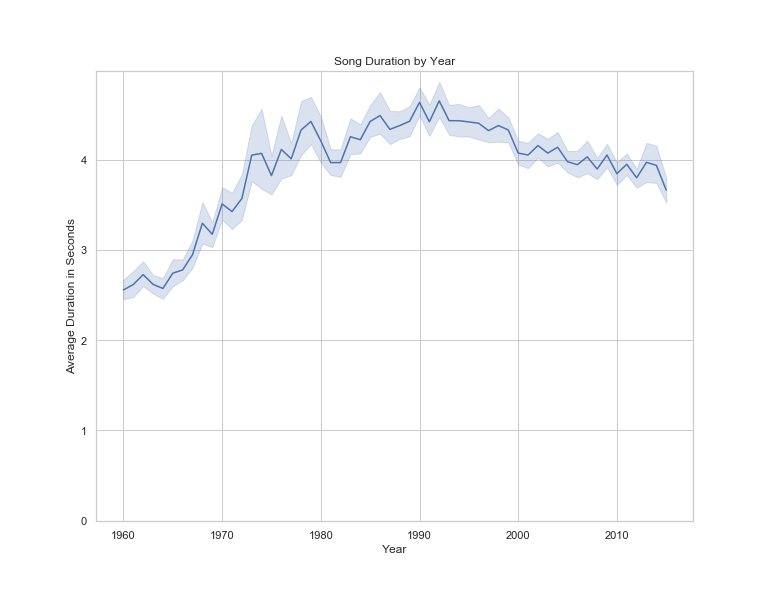
\includegraphics[width=\textwidth, height=\textheight,keepaspectratio]{average_duration_by_year.png}
    \par
}

\end{frame}

\begin{frame}
\frametitle{Songs are Getting Louder}

{
    \centering
    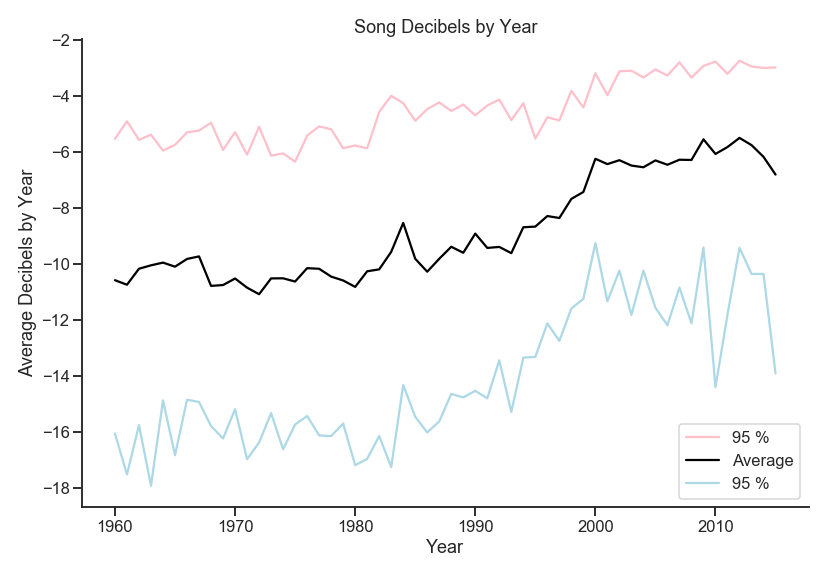
\includegraphics[width=\textwidth, height=\textheight,keepaspectratio]{average_decibels_by_year.png}
    \par
}

\end{frame}

\begin{frame}
\frametitle{More Words per Minute (Rap's Influence?)}

{
    \centering
    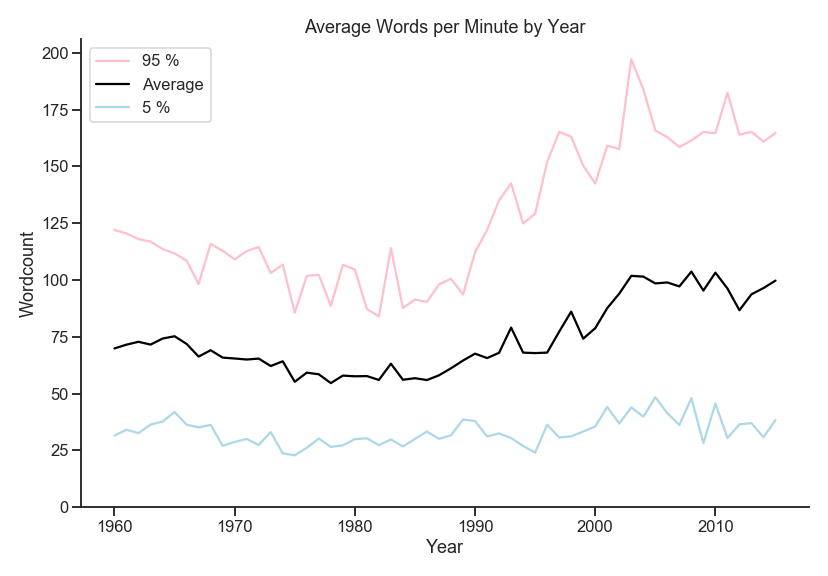
\includegraphics[width=\textwidth, height=\textheight,keepaspectratio]{average_words_per_minute_by_year.png}
    \par
}

\end{frame}

\begin{frame}
\frametitle{Death of Acousticness/Rise of Dance Music}

{
    \centering
    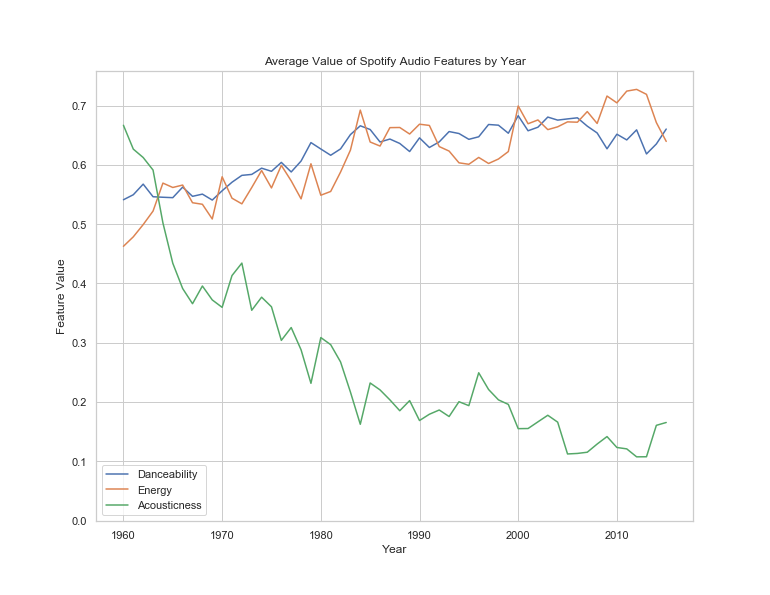
\includegraphics[width=\textwidth, height=\textheight,keepaspectratio]{the_victory_of_electric_music.png}
    \par
}

\end{frame}

\begin{frame}
\frametitle{Audio Features Show Decreasing Positivity}

{
    \centering
    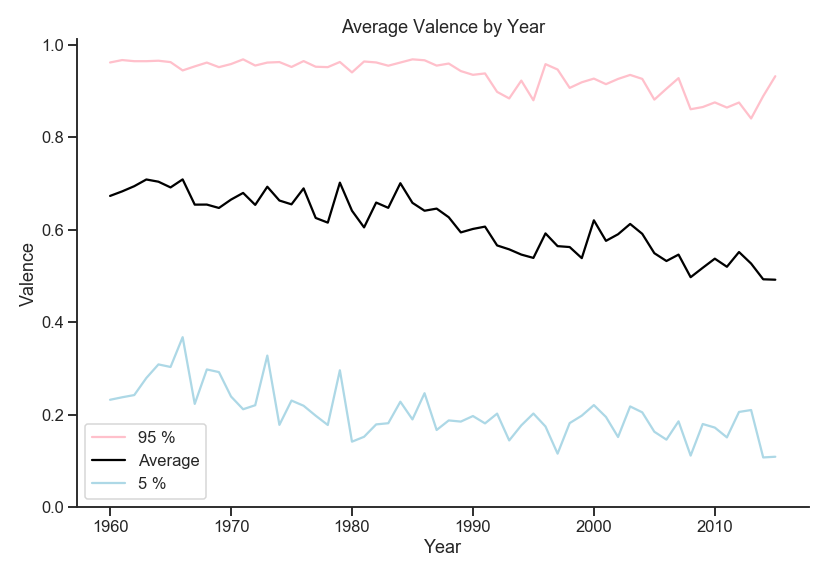
\includegraphics[width=\textwidth, height=\textheight,keepaspectratio]{spotify_valence_by_year.png}
    \par
}

\end{frame}

%------------------------------------------------
\subsection{Lyrics Sentiment}

\begin{frame}
\frametitle{Results}

\LARGE{\centerline{Lyrics Sentiment}}

\end{frame}
%------------------------------------------------

\begin{frame}
\frametitle{Afinn Positive Sentiment is in Decline}

{
    \centering
    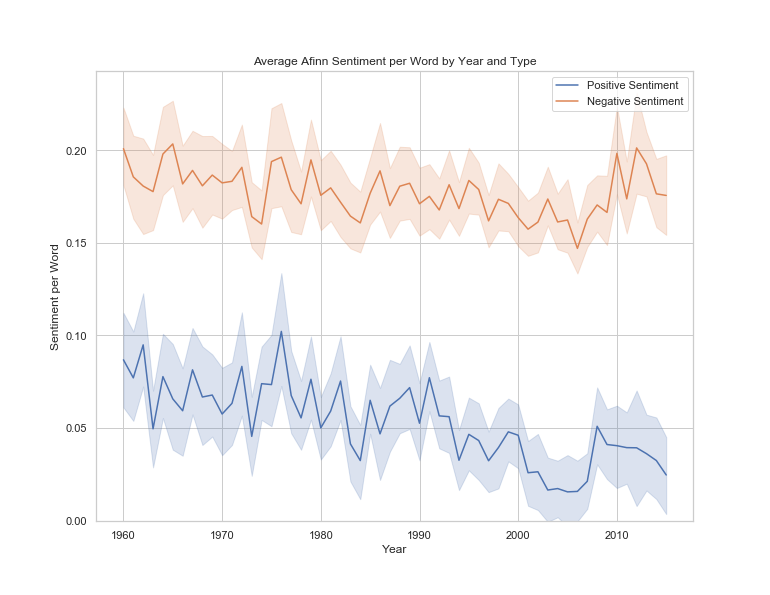
\includegraphics[width=\textwidth, height=\textheight,keepaspectratio]{average_afinn_sentiment_by_year.png}
    \par
}

\end{frame}

\begin{frame}
\frametitle{NRC Shows the Same}

{
    \centering
    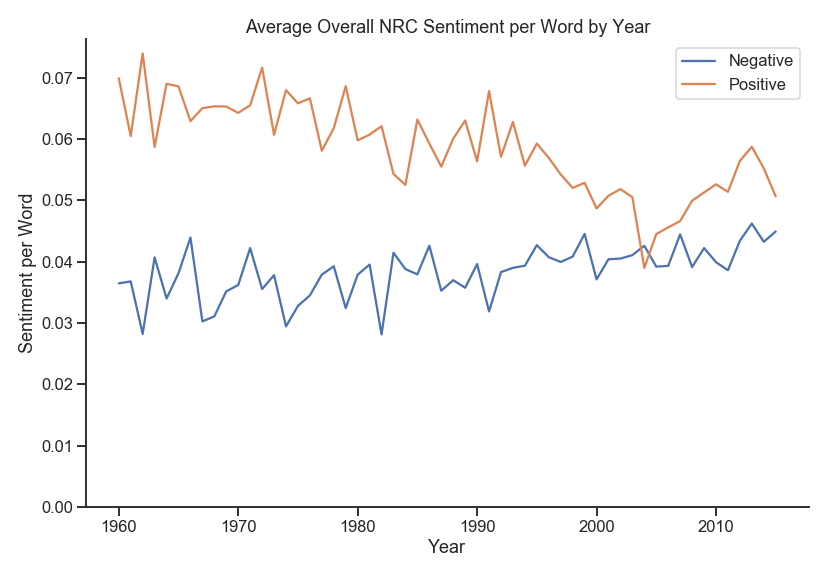
\includegraphics[width=\textwidth, height=\textheight,keepaspectratio]{average_nrc_emotions_overall_by_year.png}
    \par
}

\end{frame}

\begin{frame}
\frametitle{This Is Because There Is Less Joy In Lyrics}

{
    \centering
    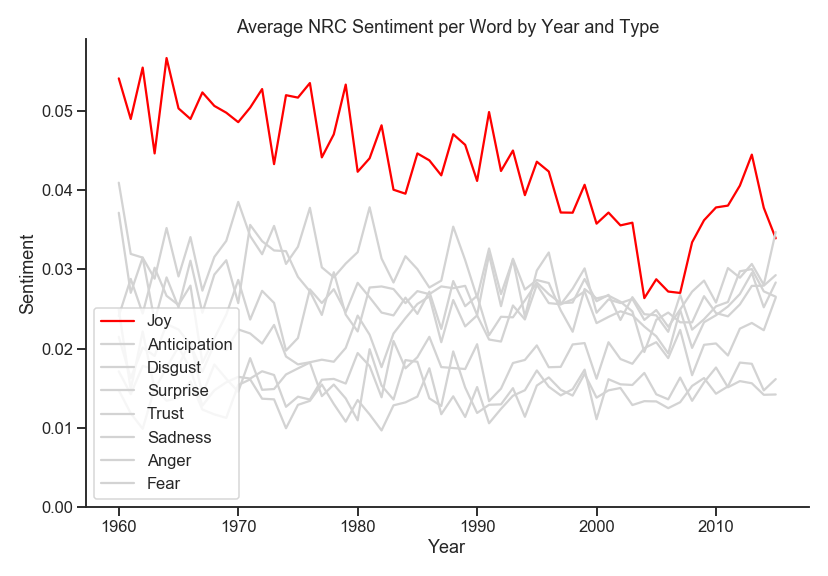
\includegraphics[width=\textwidth, height=\textheight,keepaspectratio]{average_nrc_sentiment_by_year.png}
    \par
}

\end{frame}

\begin{frame}
\frametitle{Indexed Sentiment Goes Down}

{
    \centering
    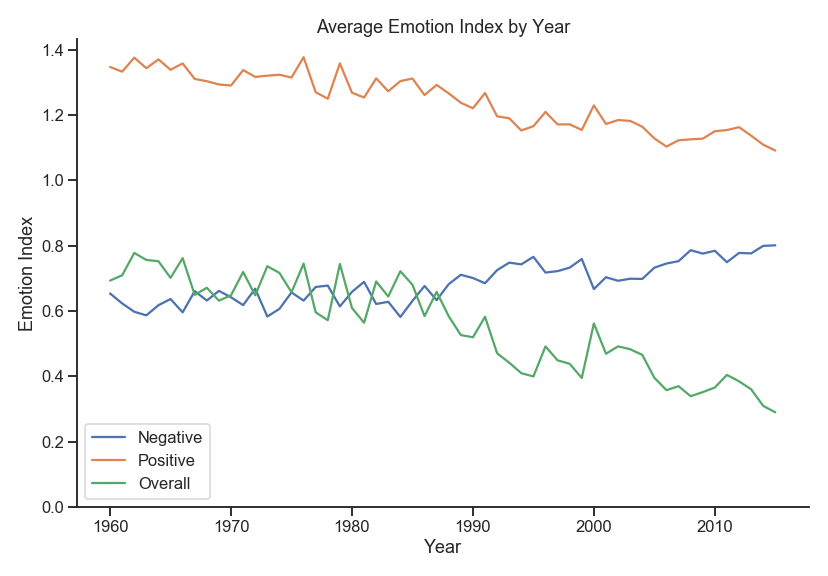
\includegraphics[width=\textwidth, height=\textheight,keepaspectratio]{emotion_index_by_year.png}
    \par
}

\end{frame}

%------------------------------------------------
\section{Conclusion}
%------------------------------------------------

\begin{frame}
\frametitle{Conclusions}

\textbf{Hits have become:}
\medskip
\begin{enumerate}
    \item Longer
    \item Louder
    \item More danceable
    \item Less happy (just from audio features)
\end{enumerate}
\bigskip

\textbf{Lyrics of the hits have become:}
\medskip
\begin{enumerate}
    \item Longer
    \item Less positive (less joy and positiveness)
\end{enumerate}

\end{frame}

\begin{frame}
    \frametitle{Just For Fun}
    \begin{itemize}
        \item Most positive song: Hank Ballard and The Midnighters - Finger Poppin' Time, 1960
        \item Most negative song: Tyga - Rack City, 2012
        \item Most words: Eminem - Rap God, 2013
        \item Most unique words: Eminem - Rap God, 2013
    \end{itemize}
\end{frame}
\begin{frame}
\frametitle{The End}

\LARGE{\centerline{Questions?}}

\end{frame}

%----------------------------------------------------------------------------------------

\end{document}
